\chapter{Simulation of the System}
To be able to verify the controller and the general control structure, the system was simulated using MATLAB and Simulink. This meant that a mathematical model of the hexacopter needed to be derived and that the low level controllers and thrust allocation of the APM needed to be simulated using some approximations and assumtions on its behaviour. The different models are derived below, then they are put together to a full system including the controller to be able to put the controller to the test.
\section{Mathematical Model of the Hexacopter}
\begin{figure}[H]
\centering
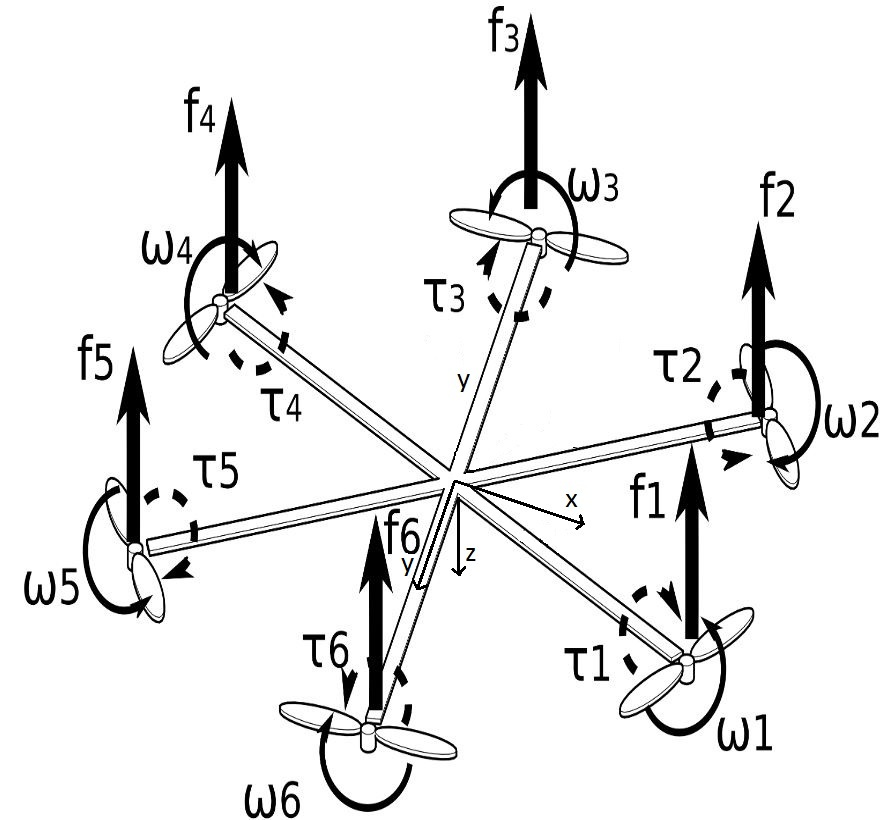
\includegraphics[width = 8cm]{fig/model.jpg}
\caption{Model of hexacopter \textit{Courtesy of \citep{model}}}
\label{model}
\end{figure}
To model the dynamics of the hexacopter equations (\ref{RB}) and (\ref{RB2}) are used. The key component that needs to be derived is the torque vector $\boldsymbol{\tau}_{RB}$, which is expressed in the BODY-frame. The thrust from each propeller is according to \citep{model} expressed as a lift constant times the squared angular speed of the propeller. In addition they approximate the moment caused around the propeller axis as a drag constant times the squared angular speed of the propeller plus the inertia moment of the propeller times the angular acceleration of the propeller. This is shown in equations (\ref{model2}) and (\ref{model3}).
\begin{eqnarray}
\boldsymbol{f}_i = \begin{bmatrix}
0 & 0 & k\omega_i^2
\label{model2}
\end{bmatrix}^T\\
\tau_{M_i} = b\omega_i^2 + I_{M_i}\dot{\omega}_i
\label{model3}
\end{eqnarray} 
Where $k$ is the lift constant, $b$ is the drag constant, $I_m$ is the inertia moment of a propeller and $\omega_i$ is the angular speed of propeller $i$. These equations and some simple geometry gives the following force and moment balances, where $\phi$ is the roll angle, $\theta$ is the pitch angle and $l$ is the length of the arm from the center of gravity to the center of the propeller.
\begin{eqnarray}
\boldsymbol{\tau}_{RB} = \begin{bmatrix}
-mg\sin(\theta)\\
mg\cos(\theta)\sin(\phi)\\
mg\cos(\theta)\cos(\phi) - k \sum_{i=1}^6\omega_i^2\\
kl(-\dfrac{1}{2}\omega_1^2 +\dfrac{1}{2}\omega_2^2 + \omega_3^2 +\dfrac{1}{2}\omega_4^2 -\dfrac{1}{2}\omega_5^2 -\omega_6^2\\
\dfrac{\sqrt{3}}{2}kl(\omega_1^2 + \omega_2^2 - \omega_4^2 - \omega_5^2)\\
b(\omega_1^2 - \omega_2^2 + \omega_3^2 - \omega_4^2 + \omega_5^2 - \omega_6^2) + I_m(\dot{\omega}_1^2 + \dot{\omega}_2^2 + \dot{\omega}_3^2 + \dot{\omega}_4^2 + \dot{\omega}_5^2 + \dot{\omega}_6^2)
\end{bmatrix}
\label{tau}
\end{eqnarray}
Not considering the different parameters, all the information needed to use equations (\ref{RB}) and (\ref{RB2}) are present, which gives.
\begin{eqnarray}
\dot{\boldsymbol{\nu}} = \boldsymbol{M}_{RB}^{-1}(\boldsymbol{\tau}_{RB} - \boldsymbol{C}_{RB}(\boldsymbol{\nu})\boldsymbol{\nu})
\end{eqnarray}
This equation is then transformed to the NED frame using the rotation matrix in equation (\ref{R_ned}) and the transformation matrix in equation (\ref{trans}) as shown in equation (\ref{eta}).
\begin{eqnarray}
\boldsymbol{\eta} = \begin{bmatrix}
\boldsymbol{R}_b^n(\boldsymbol{\Theta}_{nb}) & \boldsymbol{0}_{3 \times 3}\\
\boldsymbol{0}_{3 \times 3} & \boldsymbol{T}_\Theta(\boldsymbol{\Theta}_{nb})
\end{bmatrix}
\boldsymbol{\nu}
\label{eta}
\end{eqnarray}
Where $\boldsymbol{\eta} = [\boldsymbol{p}^n, \boldsymbol{\Theta}_{nb}]^T$ is the position in NED and the Euler angles.
\section{Simulation of Low Level Controllers and Thrust Allocation in the APM}
The attitude controllers in the APM are approximated as PD-controllers. One must assume that the controllers of the APM follows the references given, PD-controllers will do this, hence this is a fair approximation. The height controller of the APM is approximated as a PID-controller.\\
\newline
%The purpose of the thrust allocation algorithm is to convert desired force or moments in the different degrees of freedom into desired thrust from the different motors. A way to manage this is proposed and derived in \citep{sorensen} is rendered here.\\
%\newline
%The relationship between the control vector
The purpose of the thrust allocation algorithm is to convert desired force or moments in the different degrees of freedom into desired thrust from the different motors. The control vector given by the height and attitude controllers will contain desired thrust in negative z-direction and desired moments around the different axes. This vector is given by $\boldsymbol{\tau}_c = [T\; \tau_{\phi_c}\; \tau_{\theta_c}\; \tau_{\psi_c}]^T$. Using equation (\ref{tau}) combined with the control vector gives the following relationship.
\begin{eqnarray}
\boldsymbol{\tau}_{c} &=& \begin{bmatrix}
k & k & k & k & k & k\\
-\dfrac{1}{2}kl & \dfrac{1}{2}kl & kl & \dfrac{1}{2}kl & -\dfrac{1}{2}kl & -kl\\
\dfrac{\sqrt{3}}{2}kl & \dfrac{\sqrt{3}}{2}kl & 0 & -\dfrac{\sqrt{3}}{2}kl & -\dfrac{\sqrt{3}}{2}kl & 0\\
b & -b & b & -b & b & -b
\end{bmatrix}
\begin{bmatrix}
\omega_1^2\\
\omega_2^2\\
\omega_3^2\\
\omega_4^2\\
\omega_5^2\\
\omega_6^2
\end{bmatrix}
= \boldsymbol{A}\boldsymbol{u}\\
\boldsymbol{u} &=& \boldsymbol{A}^+\boldsymbol{\tau}_c \label{u_motor}\\
\boldsymbol{A}^+ &=& \boldsymbol{A}^T(\boldsymbol{A}\boldsymbol{A}^T)^{-1}\label{pseudo}
\end{eqnarray}
The desired input to each motor is calculated using equation (\ref{u_motor}), where the pseudo inverse of $\boldsymbol{A}$ is calculated as shown in equation (\ref{pseudo}).
\section{Simulation of the Camera Algorithm}
To simulate the measurements from the camera, the algorithm given in Section \ref{node} is used to find the position of each of the corners of the camera frame. Then a ray casting algorithm is used to determine if the position of the sensor node is within the camera frame. The ray casting algorithm is outside the scope of this report.\\
\newline
If the sensor node is within the camera frame, perfect measurements of both node position in relation to the hexacopter and the heading of the node are sent back to the control algorithm.
\section{Simulink Model}
All the components for the simulator explained abov,e in addition to a PandaBoard component containing the controller described in the previous chapter is put together to create the Simulink model shown in Figure  \ref{simulink}.
\begin{figure}[H]
\centering
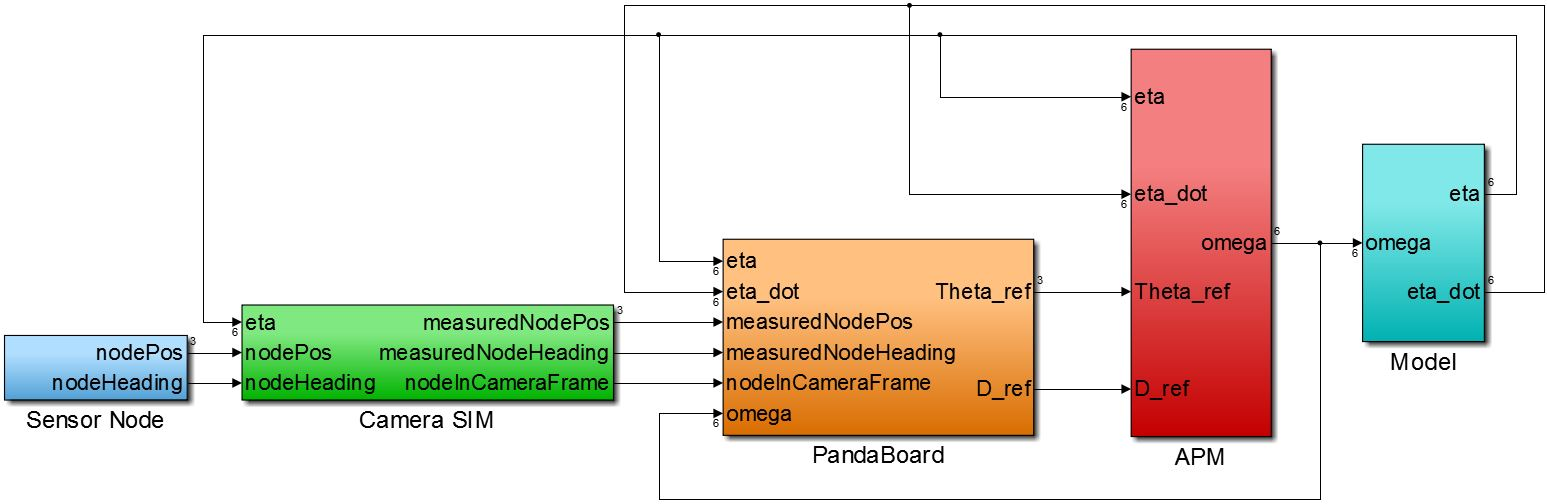
\includegraphics[width = 18cm]{fig/simulink.jpg}
\caption{Simulink}
\label{simulink}
\end{figure}
\section{Test of Controller}
The main scenario simulated is as close to the lab tests that will be conducted as possible. As the main challenge of the hexacopter controller is the pickup phase, the simulation will focus on this phase. In each of the simulations the hexacopter ramps up from a ground start to a height of 4 m. The sensor node is assumed to be lying 0.5 m North and 0.5 m East of the starting point. As the  hexacopter is flying the simulated camera will give measurements of the position of the sensor node, but only if the sensor node would have been in the camera frame. If the camera is unable to spot the sensor node, the position reference used for the controller will be the current position. The hexacopter will also try to maintain the same heading as the sensor node. If the sensor node is in the camera frame, the reference heading for the hexacopter will be updated, if the view of the sensor node is lost, the reference will be the last measured node heading\\
\newline
Three scenarios will be simulated, first a simulation with no disturbances, then a simulation with constant disturbance and lastly a simulation with varying disturbances.
\subsection{Simulation Without Disturbances}
The scenario was first simulated using the proposed controller from equation (\ref{u}) without any disturbances present.
\subsubsection{Results}
The North-East-Down position of the sensor node is plotted in Figure \ref{posNoDisturbance}. It can be seen from the figure how the reference position is updated when the camera spots the sensor node. And one should also note that the hexacopter ramps down all the way to the sensor node without loosing sight of the sensor node. 
\begin{figure}[H]
\centering
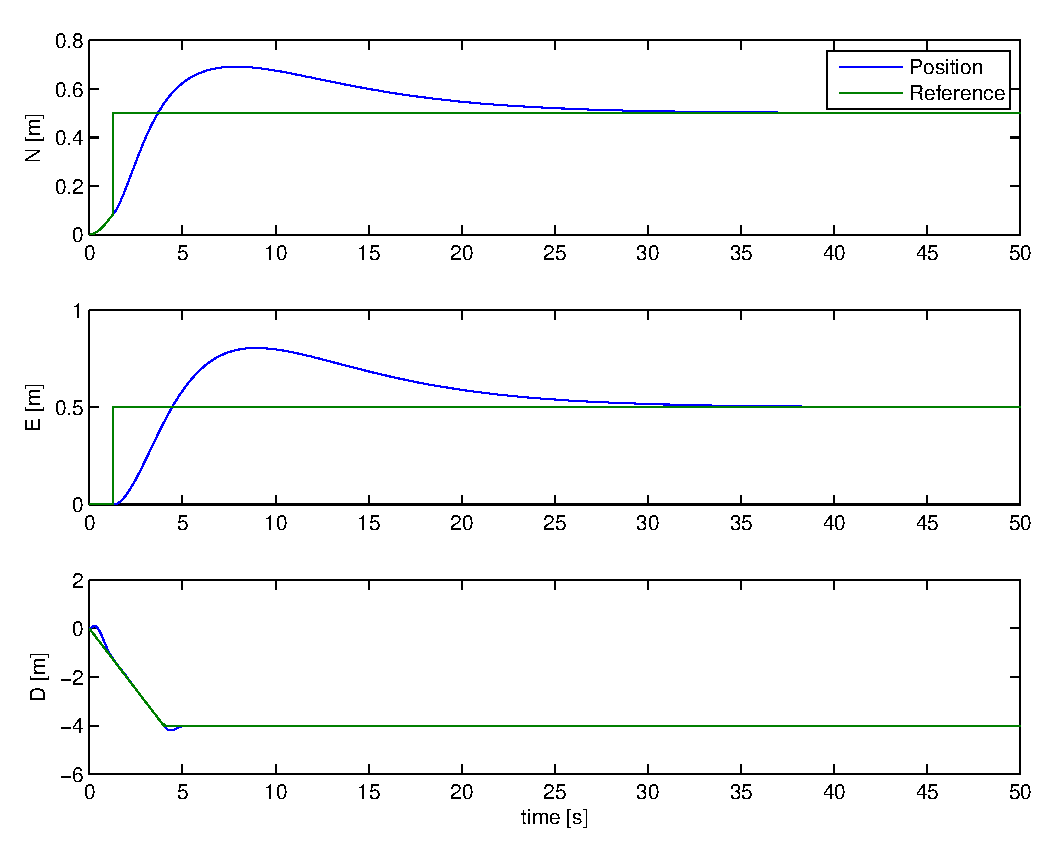
\includegraphics[width = 12cm]{fig/plots/simulation/positionNoDisturbance.eps}
\caption{North-East-Down position of the hexacopter}
\label{posNoDisturbance}
\end{figure}
\noindent
Figure \ref{posFrameNoDisturbance} shows the the North-East position of the hexacopter and the sensor node. It also shows the camera frame and whether the node is spotted by the camera or not. It can also be seen from this plot how the hexacopter yaws to keep the same heading as the sensor node (this can be seen even better from attitude plots shown in  Appendix A). 
\begin{figure}[H]
\centering
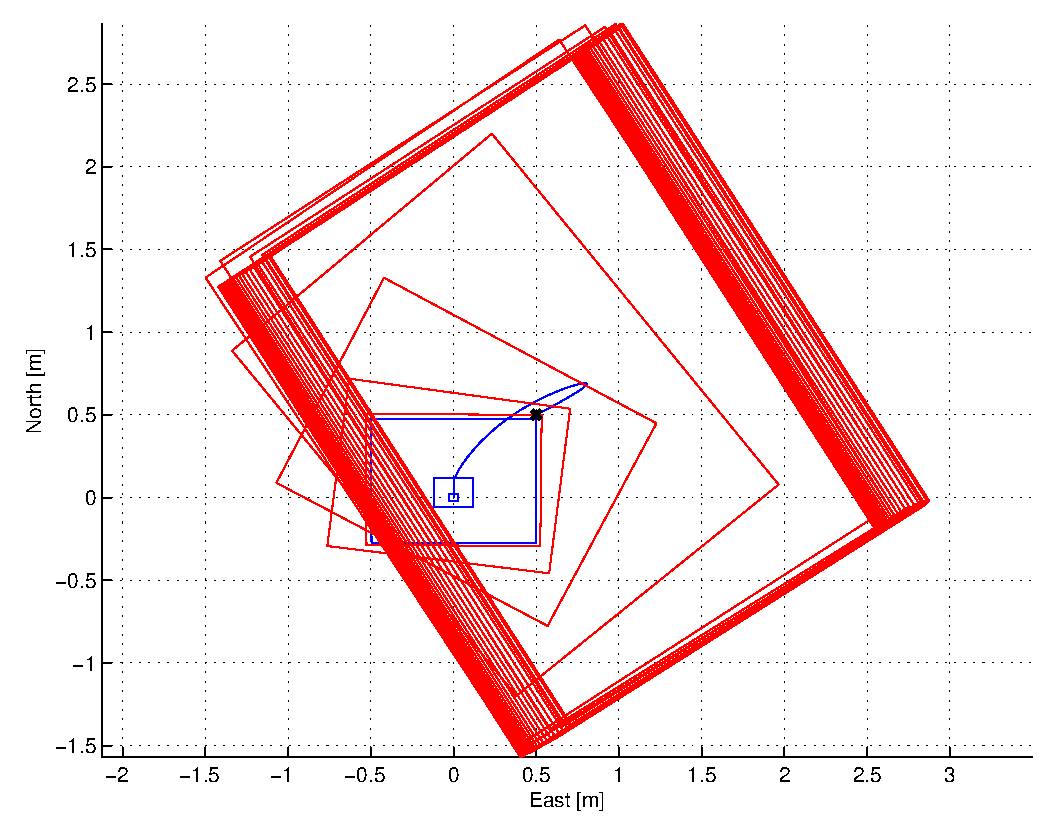
\includegraphics[width = 12cm]{fig/plots/simulation/positionFrameNoDisturbance.eps}
\caption{North-East-Down position of the hexacopter, sensor node and camera frame}
\label{posFrameNoDisturbance}
\end{figure}
\subsubsection{Discussion}
The hexacopter is able to lower itself down on the exact spot of the sensor node without loosing sight of the sensor node. This is very promising results, although some early tests in the lab showed that the controller used in this simulation would give some stationary deviations. The lab tests were conducted inside so wind played no part in this error. The error is probably due to unbalances of the hexacopter and inaccuracies of the low level controllers of the APM. Hence integral action was added to the controller. A simulation with constant disturbance and integral action follows.
\subsection{Simulation With Constant Disturbances}
The disturbance added could for instance represent a wind affecting the hexacopter with a force of 0.5 N in North-direction.
\subsubsection{Results}
As can be seen from Figure \ref{posFrameDisturbance} and Figure \ref{posFrameDisturbance} the hexacopter overshoots the reference position. The controller is able to cancel out the disturbance and make the hexacopter descend upon the sensor node.
\begin{figure}[H]
\centering
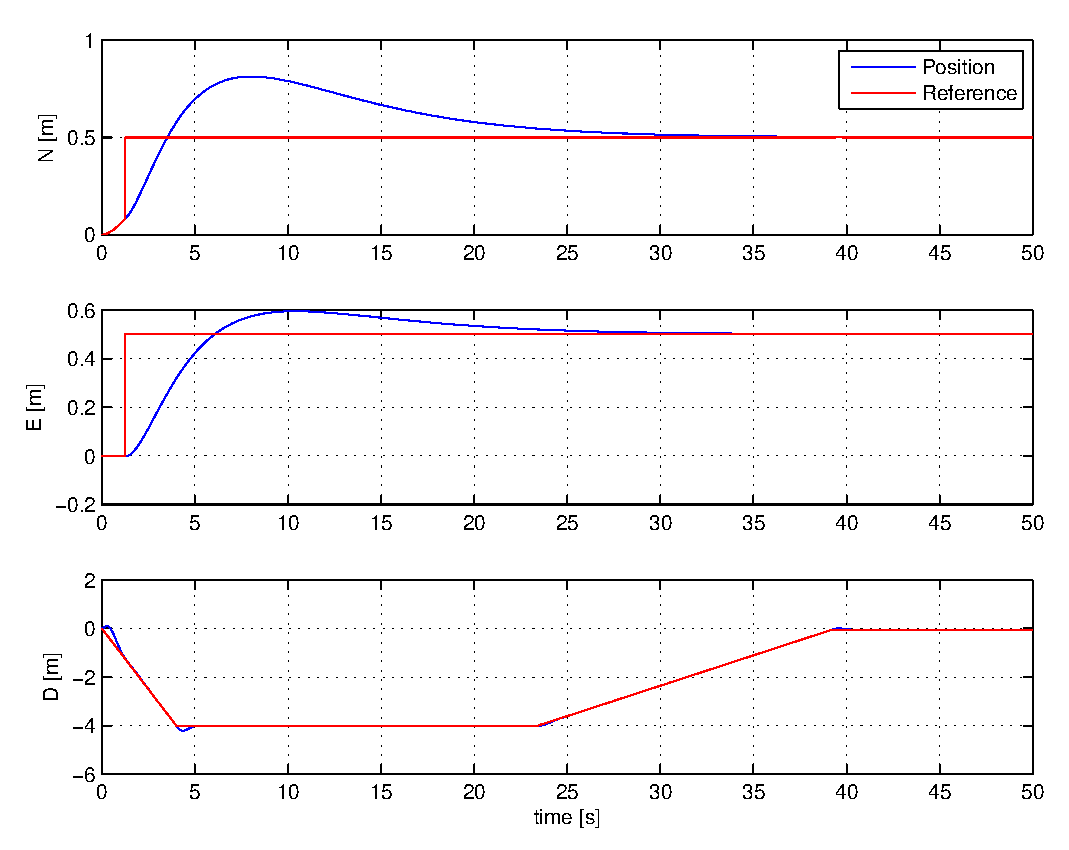
\includegraphics[width = 12cm]{fig/plots/simulation/positionDisturbance.eps}
\caption{North-East-Down position of the hexacopter}
\label{posDisturbance}
\end{figure}
\begin{figure}[H]
\centering
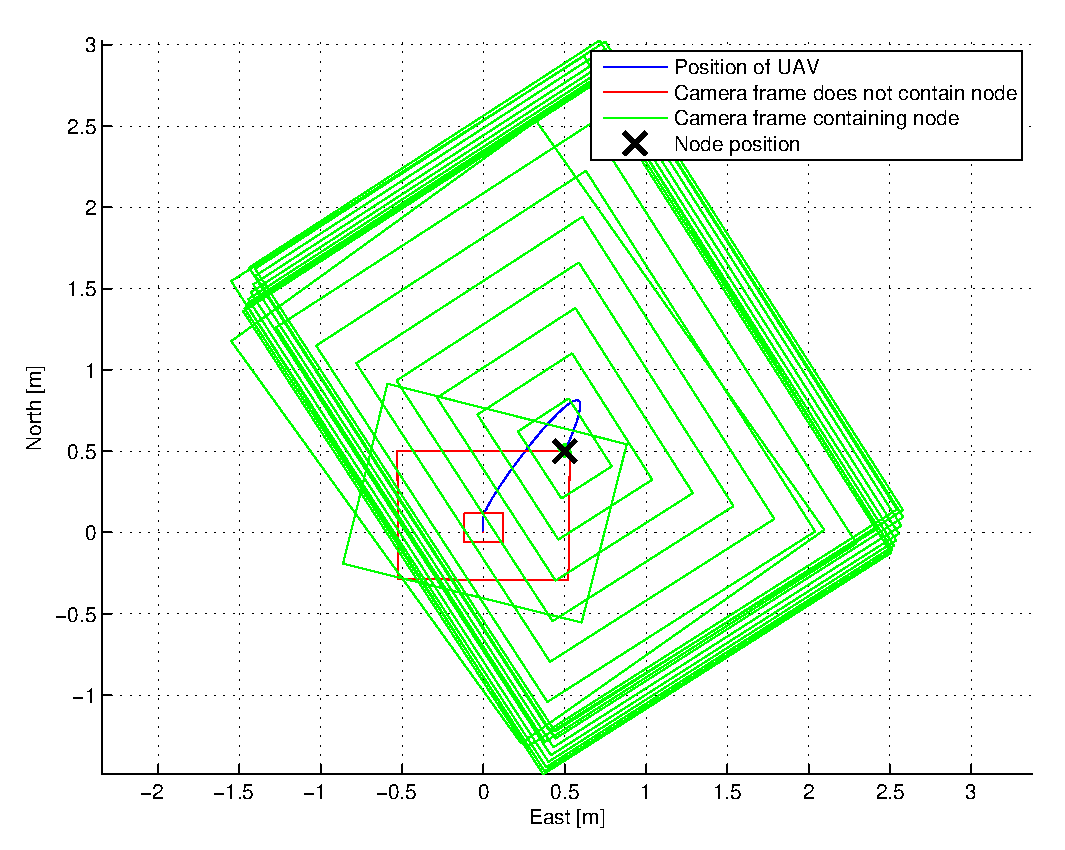
\includegraphics[width = 12cm]{fig/plots/simulation/positionFrameDisturbance.eps}
\caption{North-East-Down position of the hexacopter, sensor node and camera frame}
\label{posFrameDisturbance}
\end{figure}
\subsubsection{Discussion}
The overshoot of the position reference is due to the I-term of the controller and is quite natural due to the step in reference position. The fact that the disturbances is working in North-direction will also lead to an overshoot in North-direction, due to the added forces in that direction. The controller is able to correct for the disturbance and descend upon the sensor node, which is very good. 
\subsection{Simulation With Varying Disturbances}
The controller is tested in simulations where the disturbances are varying in both North and East-direction using integrated band limited white noise where the integral is limited by $\pm$ 1 N in both directions. The magnitude and direction of the disturbance is plotted in the appendix.
\subsubsection{Results}
The hexacopter stays approximately straight above the sensor node, and is able to lower itself a bit down towards the sensor node before it looses the sight of the node and drifts away. Both these observations are easily seen in Figures \ref{posVarDisturbance} and \ref{posFrameVarDisturbance}.
\begin{figure}[H]
\centering
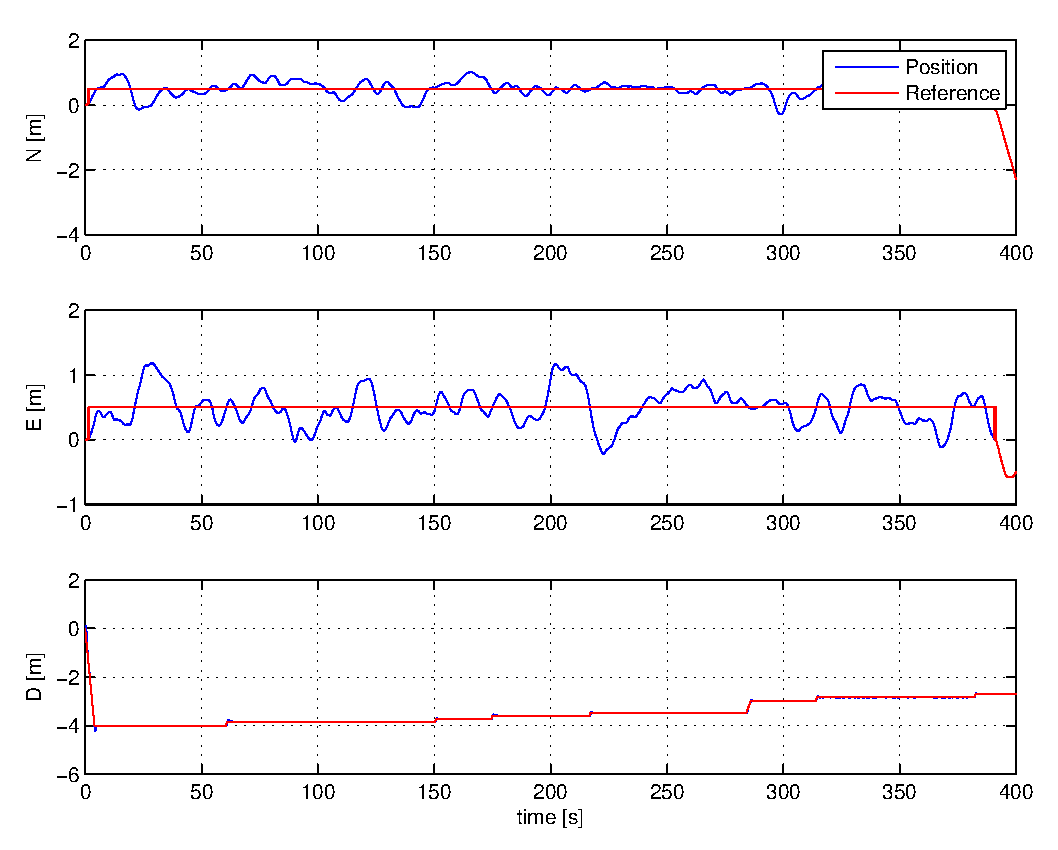
\includegraphics[width = 12cm]{fig/plots/simulation/positionVarDisturbance.eps}
\caption{North-East-Down position of the hexacopter}
\label{posVarDisturbance}
\end{figure}
\begin{figure}[H]
\centering
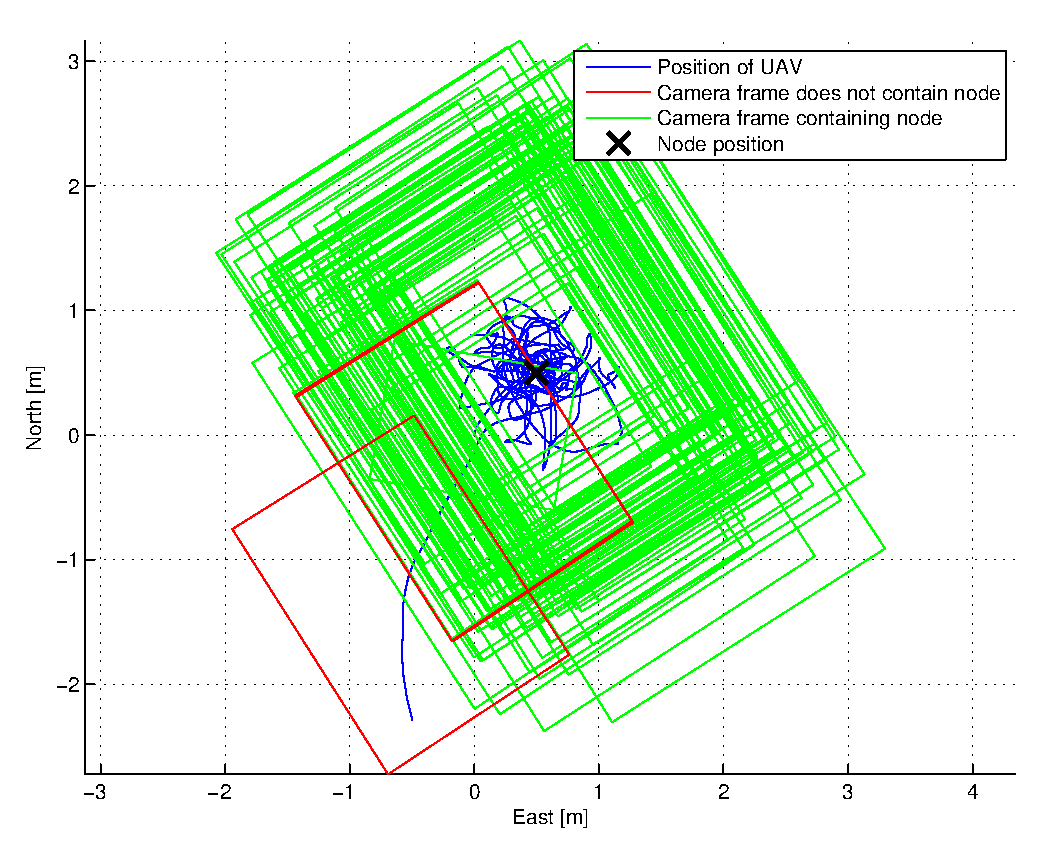
\includegraphics[width = 12cm]{fig/plots/simulation/positionFrameVarDisturbance.eps}
\caption{North-East-Down position of the hexacopter, sensor node and camera frame}
\label{posFrameVarDisturbance}
\end{figure}
\subsubsection{Discussion}
The results show that the controller is able to handle some random disturbances but sooner or later these disturbances will lead to problems where the camera will loose sight of the sensor node and then drift off. This will make pick up in such conditions impossible.
\subsection{Simulation With Constant Disturbances on the Hexacopter and Disturbances Affecting the Sensor Node}
A more realistic simulation is to simulate the system with constant disturbance, e.g. due to wind or inaccuracies in the APM. And let the sensor node be affected by some varying noise, which makes it change heading and position. The noise is modelled as random walk.
\subsubsection{Results}
As seen from Figures \ref{posNodeDisturbance} and \ref{posFrameNodeDisturbance} the hexacopter tracks both position and heading of the sensor node, and is actually able to get down to 5 cm above the sensor node before loosing sight of it and drifting off.
\begin{figure}[H]
\centering
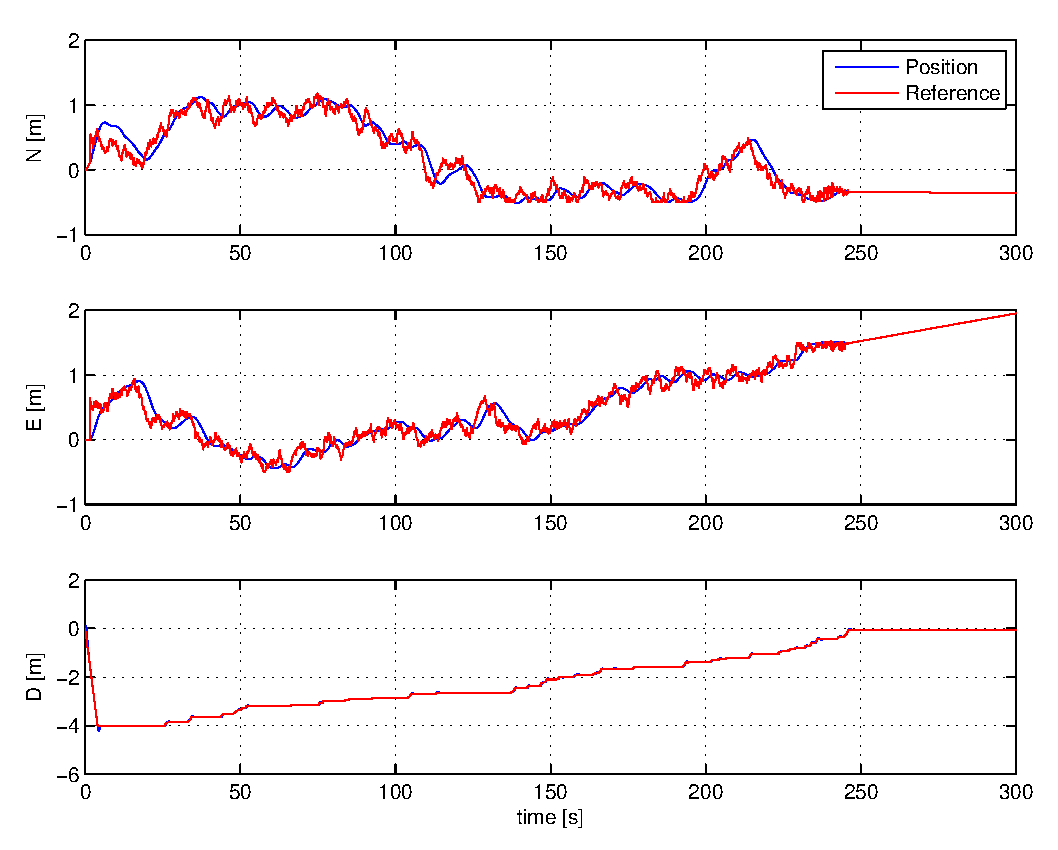
\includegraphics[width = 12cm]{fig/plots/simulation/positionNodeDisturbance.eps}
\caption{North-East-Down position of the hexacopter}
\label{posNodeDisturbance}
\end{figure}
\begin{figure}[H]
\centering
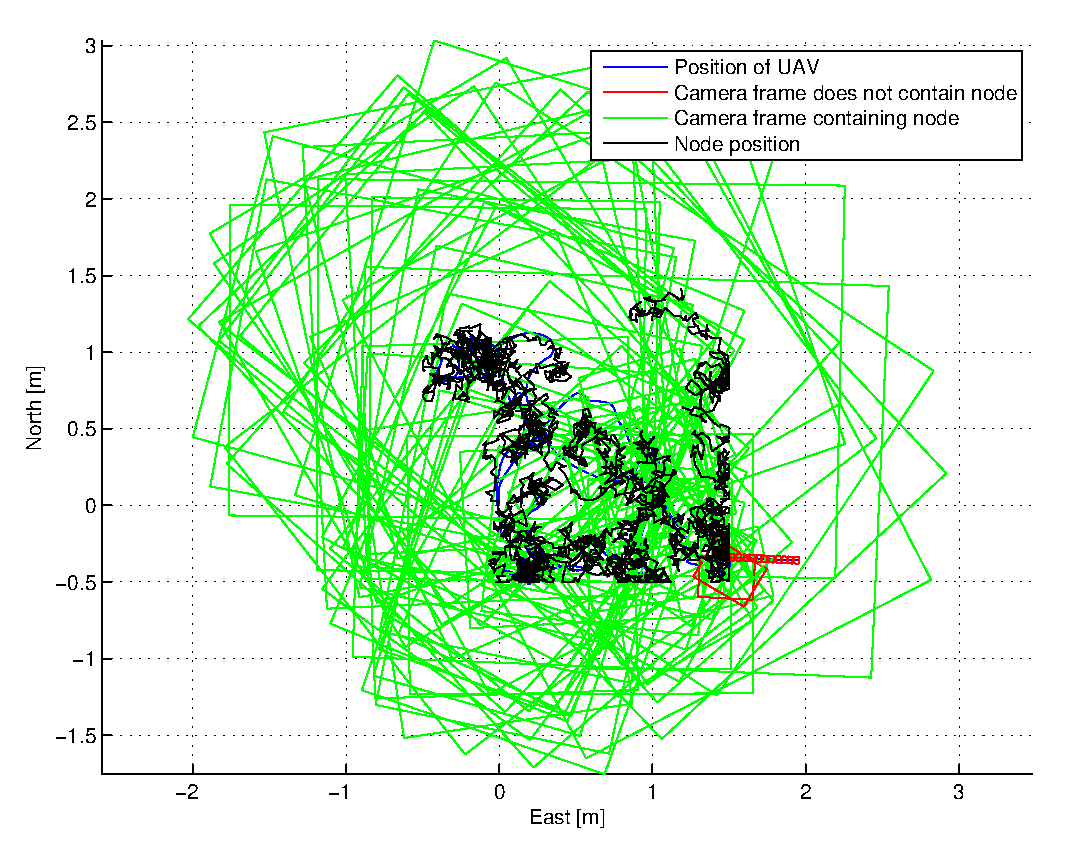
\includegraphics[width = 12cm]{fig/plots/simulation/positionFrameNodeDisturbance.eps}
\caption{North-East-Down position of the hexacopter, sensor node and camera frame} 
\label{posFrameNodeDisturbance}
\end{figure}
\subsubsection{Discussion}
The hexacopters abilities to track the sensor nodes position and heading is quite promising. The main issue that is revealed is the need for some way to get back to the previous position where the sensor node was spotted last. The simulations have also shown that this setup is not able to handle rough weather conditions, meaning that operation should be limited to days with only small waves and little wind.